% Adjust these for the path of the theme and its graphics, relative to this file
%\usepackage{beamerthemeFalmouthGamesAcademy}
\usepackage{../../beamerthemeFalmouthGamesAcademy}
\usepackage{multimedia}
\graphicspath{ {../../} }

% For strikethrough effect
\usepackage[normalem]{ulem}
\usepackage{wasysym}

\usepackage{pdfpages}
% Default language for code listings
\lstset{language=C++,
	morekeywords={each,in,nullptr}
}

% From http://blog.virtualglobebook.com/2011/02/syntax-highlighting-c-and-glsl-source.html

\lstdefinelanguage{GLSL}
{
sensitive=true,
morekeywords=[1]{
float2, float3, float3, float2x2, float3x3, float4x4,
attribute, const, uniform, varying,
layout, centroid, flat, smooth,
noperspective, break, continue, do,
for, while, switch, case, default, if,
else, in, out, inout, float, int, void,
bool, true, false, invariant, discard,
return, mat2, mat3, mat4, mat2x2, mat2x3,
mat2x4, mat3x2, mat3x3, mat3x4, mat4x2,
mat4x3, mat4x4, vec2, vec3, vec4, ivec2,
ivec3, ivec4, bvec2, bvec3, bvec4, uint,
uvec2, uvec3, uvec4, lowp, mediump, highp,
precision, sampler1D, sampler2D, sampler3D,
samplerCube, sampler1DShadow,
sampler2DShadow, samplerCubeShadow,
sampler1DArray, sampler2DArray,
sampler1DArrayShadow, sampler2DArrayShadow,
isampler1D, isampler2D, isampler3D,
isamplerCube, isampler1DArray,
isampler2DArray, usampler1D, usampler2D,
usampler3D, usamplerCube, usampler1DArray,
usampler2DArray, sampler2DRect,
sampler2DRectShadow, isampler2DRect,
usampler2DRect, samplerBuffer,
isamplerBuffer, usamplerBuffer, sampler2DMS,
isampler2DMS, usampler2DMS,
sampler2DMSArray, isampler2DMSArray,
usampler2DMSArray, struct},
morekeywords=[2]{
radians,degrees,sin,cos,tan,asin,acos,atan,
atan,sinh,cosh,tanh,asinh,acosh,atanh,pow,
exp,log,exp2,log2,sqrt,inversesqrt,abs,sign,
floor,trunc,round,roundEven,ceil,fract,mod,modf,
min,max,clamp,mix,step,smoothstep,isnan,isinf,
floatBitsToInt,floatBitsToUint,intBitsToFloat,
uintBitsToFloat,length,distance,dot,cross,
normalize,faceforward,reflect,refract,
matrixCompMult,outerProduct,transpose,
determinant,inverse,lessThan,lessThanEqual,
greaterThan,greaterThanEqual,equal,notEqual,
any,all,not,textureSize,texture,textureProj,
textureLod,textureOffset,texelFetch,
texelFetchOffset,textureProjOffset,
textureLodOffset,textureProjLod,
textureProjLodOffset,textureGrad,
textureGradOffset,textureProjGrad,
textureProjGradOffset,texture1D,texture1DProj,
texture1DProjLod,texture2D,texture2DProj,
texture2DLod,texture2DProjLod,texture3D,
texture3DProj,texture3DLod,texture3DProjLod,
textureCube,textureCubeLod,shadow1D,shadow2D,
shadow1DProj,shadow2DProj,shadow1DLod,
shadow2DLod,shadow1DProjLod,shadow2DProjLod,
dFdx,dFdy,fwidth,noise1,noise2,noise3,noise4,
EmitVertex,EndPrimitive},
morekeywords=[3]{
gl_VertexID,gl_InstanceID,gl_Position,
gl_PointSize,gl_ClipDistance,gl_PerVertex,
gl_Layer,gl_ClipVertex,gl_FragCoord,
gl_FrontFacing,gl_ClipDistance,gl_FragColor,
gl_FragData,gl_MaxDrawBuffers,gl_FragDepth,
gl_PointCoord,gl_PrimitiveID,
gl_MaxVertexAttribs,gl_MaxVertexUniformComponents,
gl_MaxVaryingFloats,gl_MaxVaryingComponents,
gl_MaxVertexOutputComponents,
gl_MaxGeometryInputComponents,
gl_MaxGeometryOutputComponents,
gl_MaxFragmentInputComponents,
gl_MaxVertexTextureImageUnits,
gl_MaxCombinedTextureImageUnits,
gl_MaxTextureImageUnits,
gl_MaxFragmentUniformComponents,
gl_MaxDrawBuffers,gl_MaxClipDistances,
gl_MaxGeometryTextureImageUnits,
gl_MaxGeometryOutputVertices,
gl_MaxGeometryOutputVertices,
gl_MaxGeometryTotalOutputComponents,
gl_MaxGeometryUniformComponents,
gl_MaxGeometryVaryingComponents,gl_DepthRange},
morecomment=[l]{//},
morecomment=[s]{/*}{*/},
morecomment=[l][keywordstyle4]{\#},
}


% http://www.texample.net/tikz/examples/state-machine/
\usetikzlibrary{arrows,automata}

\newcommand{\modulecode}{GAM250}\newcommand{\moduletitle}{Advanced Games Programming }\newcommand{\sessionnumber}{2}

\begin{document}
\title{\sessionnumber: Graphics Programming}
\subtitle{\modulecode: \moduletitle}

\frame{\titlepage} 

\begin{frame}
	\frametitle{Learning outcomes}
	\begin{itemize}
		\item \textbf{Understand} the modern Programmable Graphics Pipeline
		\item \textbf{Understand} Unity's Material System
		\item \textbf{Write} Surface and Image Effect Shaders in Unity
	\end{itemize}
\end{frame}

\part{The Graphics Pipeline}
\frame{\partpage}

\begin{frame}{The 3D graphics pipeline}
\begin{center}
	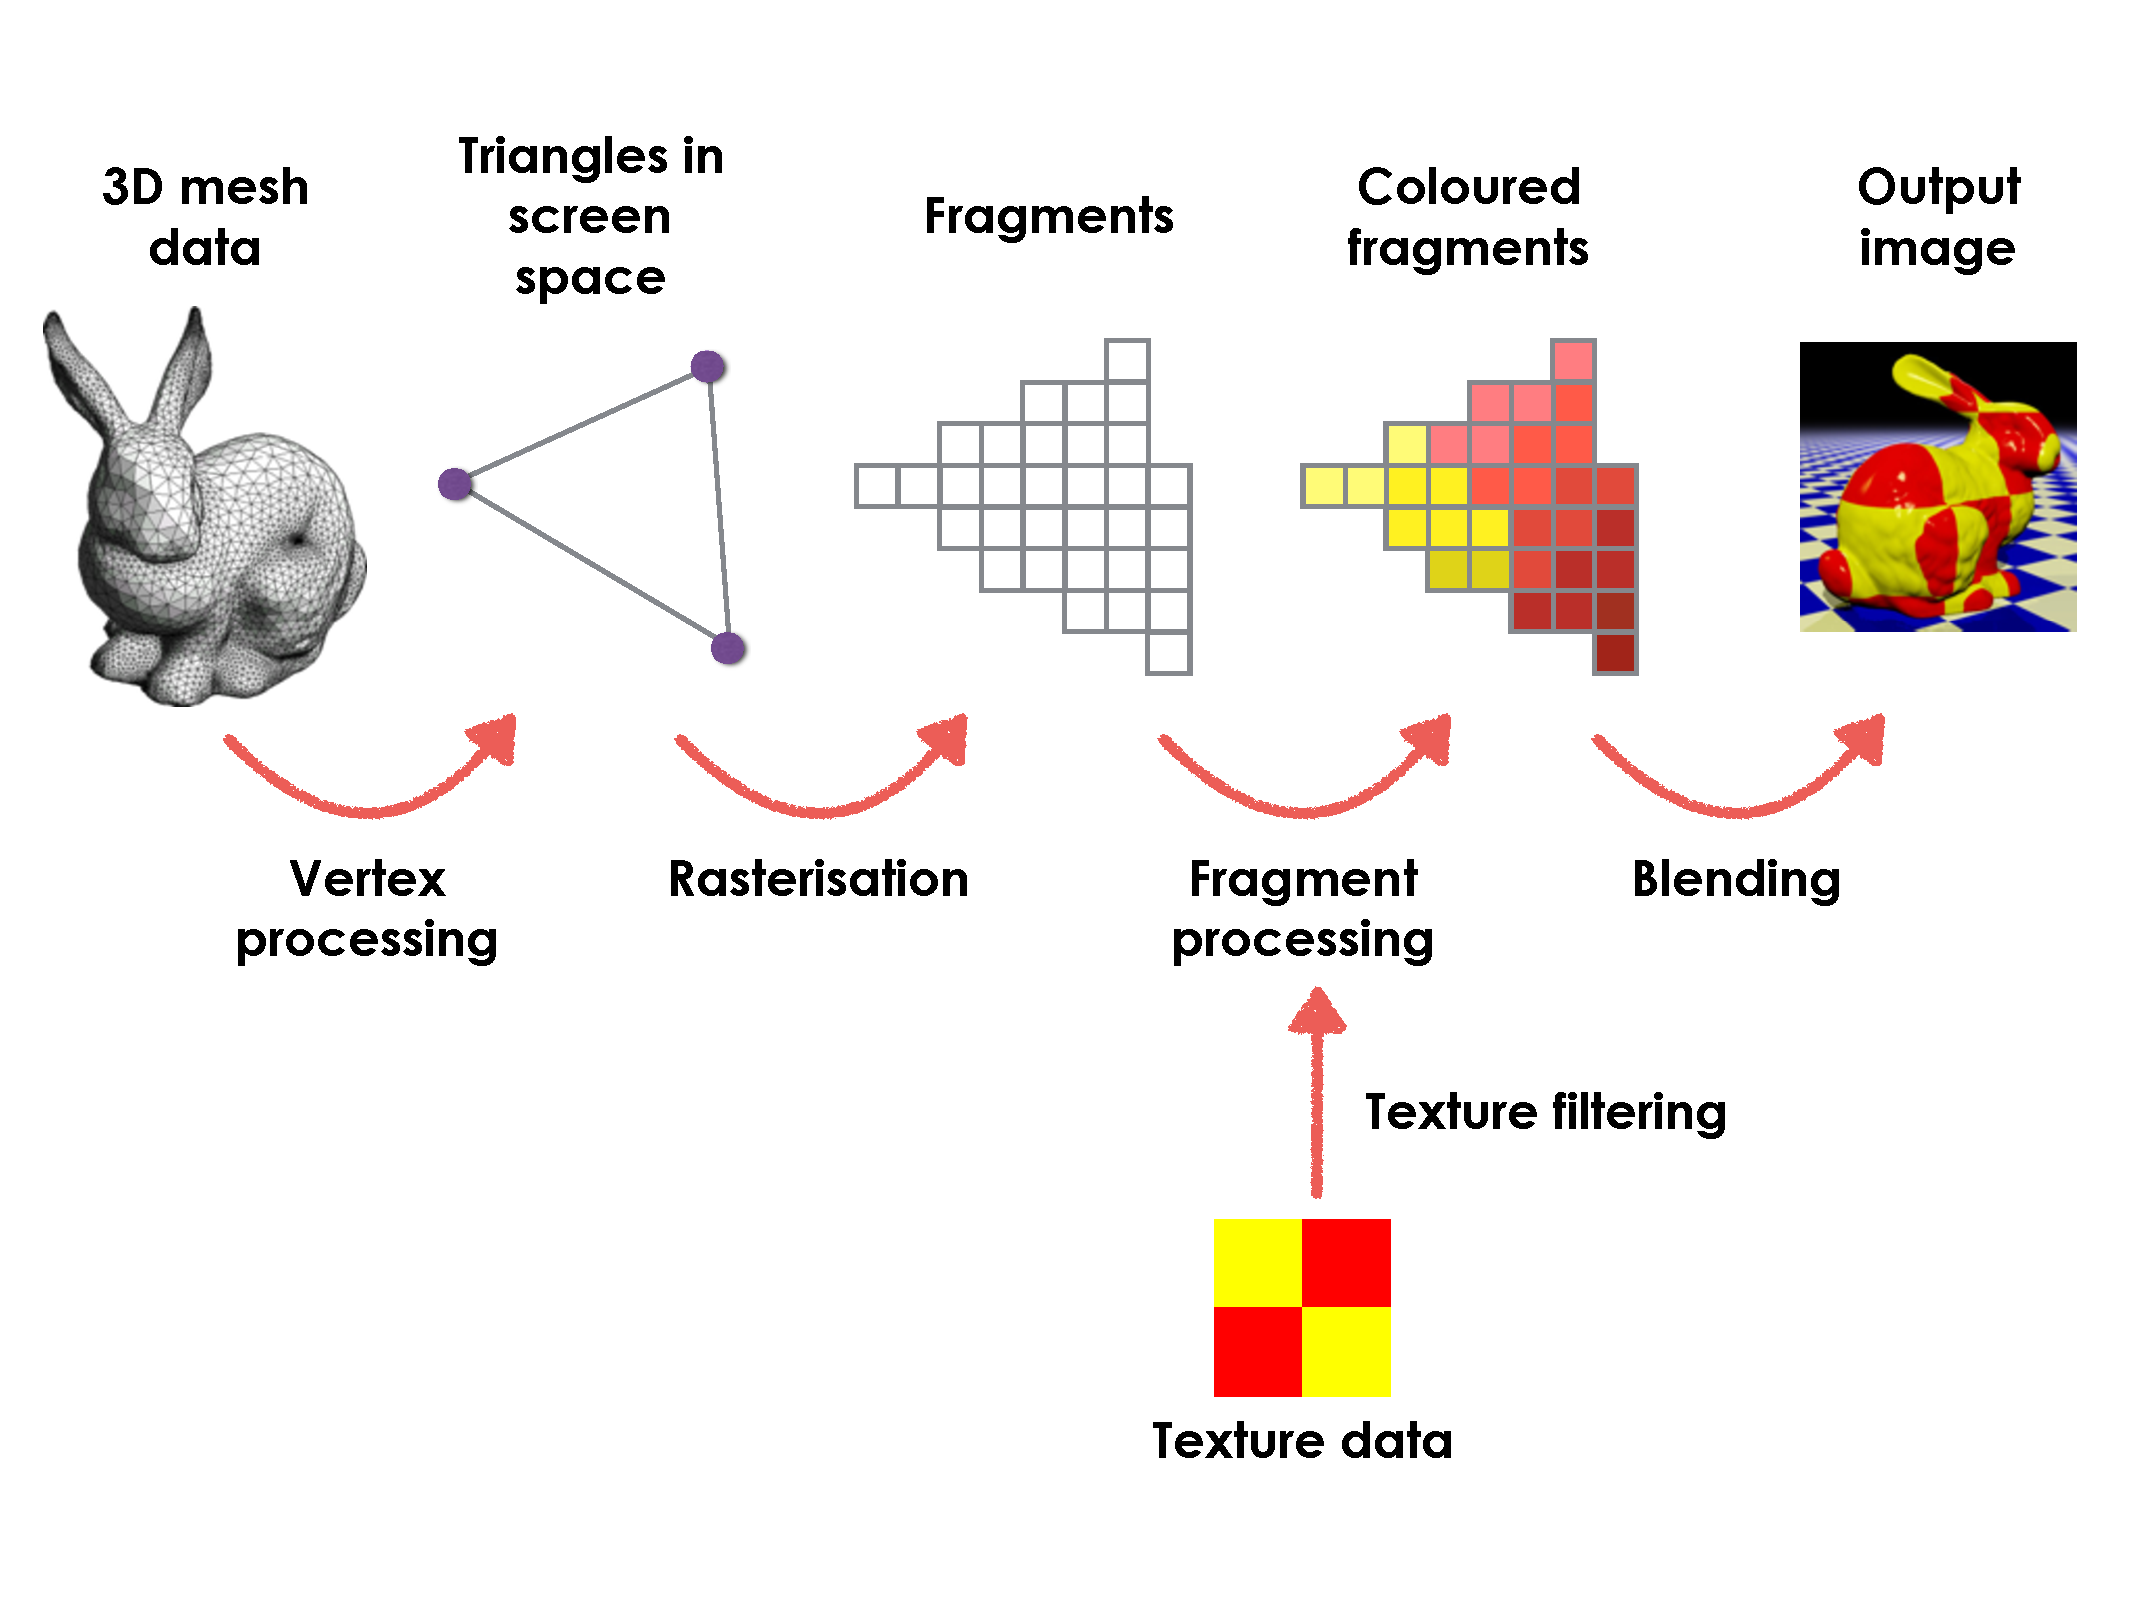
\includegraphics[height=0.7\textheight]{pipeline}
\end{center}
\end{frame}

\begin{frame}{Vertex processing}
\begin{columns}
\begin{column}{0.3\textwidth}
	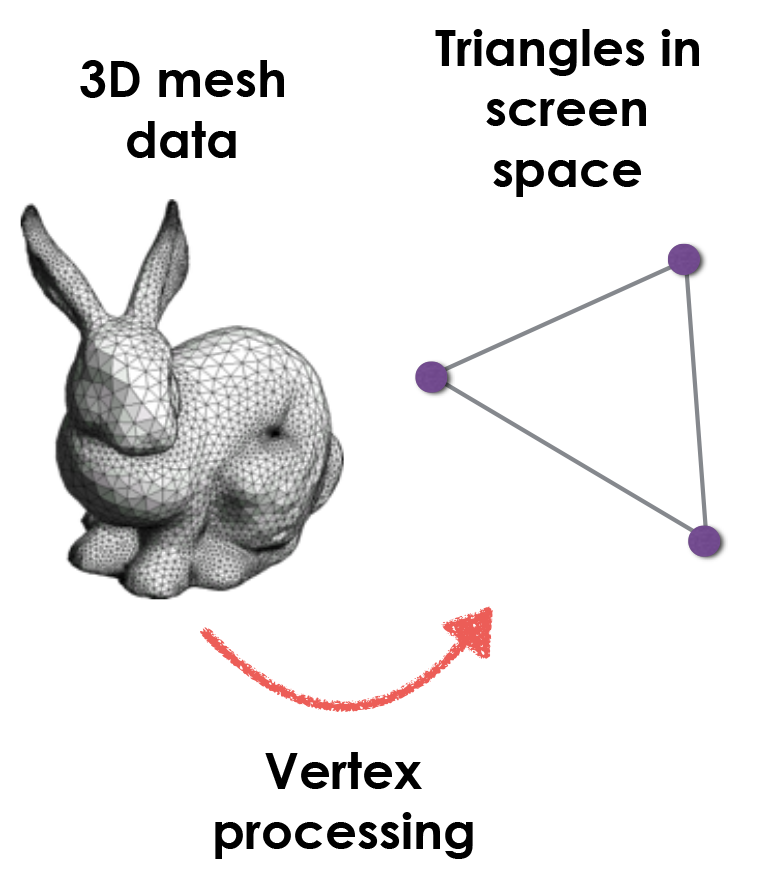
\includegraphics[width=\textwidth]{pipeline_1}
\end{column}
\begin{column}{0.65\textwidth}
	\begin{itemize}
		\pause\item Geometry is provided to the GPU as a \textbf{mesh} of \textbf{triangles}
		\pause\item Each triangle has three \textbf{vertices} specified in 3D space $(x,y,z)$
		\pause\item Vertex processor \textbf{transforms} (rotates, moves, scales) vertices
		and \textbf{projects} them into 2D screen space $(x,y)$
		\pause\item May also apply particle simulations, skeletal animations or deformations, etc.
	\end{itemize}
\end{column}
\end{columns}
\end{frame}

\begin{frame}{Rasterisation}
\begin{columns}
\begin{column}{0.3\textwidth}
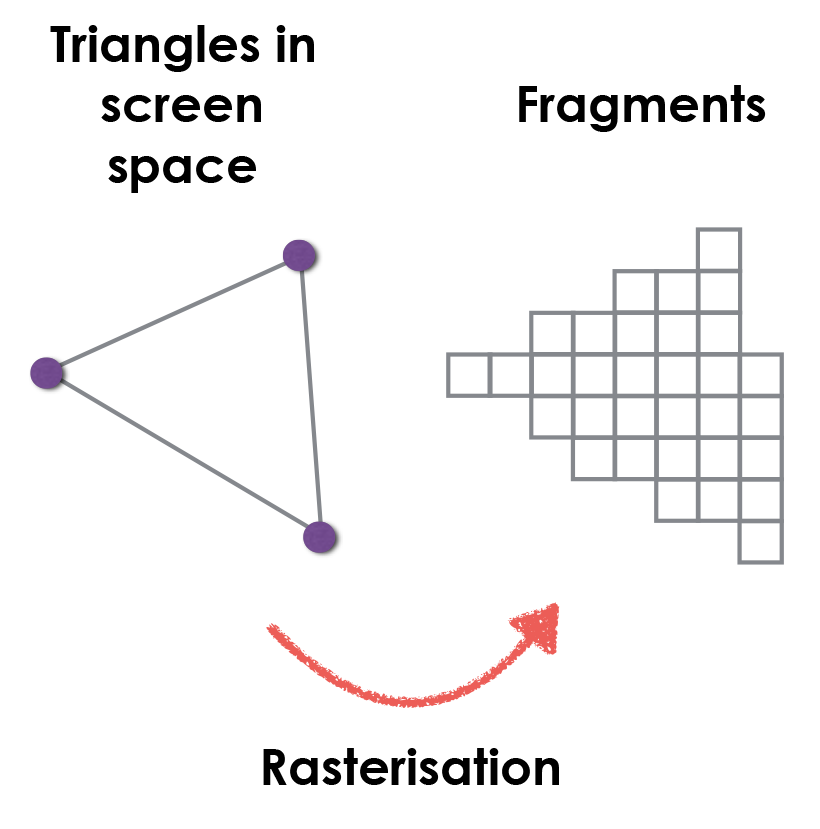
\includegraphics[width=\textwidth]{pipeline_2}
\end{column}
\begin{column}{0.65\textwidth}
\begin{itemize}
	\pause\item Determine \textbf{which fragments} are covered by the triangle
	\pause\item In practical terms, ``fragment'' = ``pixel''
	\pause\item Vertex processor can associate \textbf{data} with each vertex;
	this is \textbf{interpolated} across the fragments
\end{itemize}
\end{column}
\end{columns}
\end{frame}

\begin{frame}{Fragment processing}
\begin{columns}
\begin{column}{0.3\textwidth}
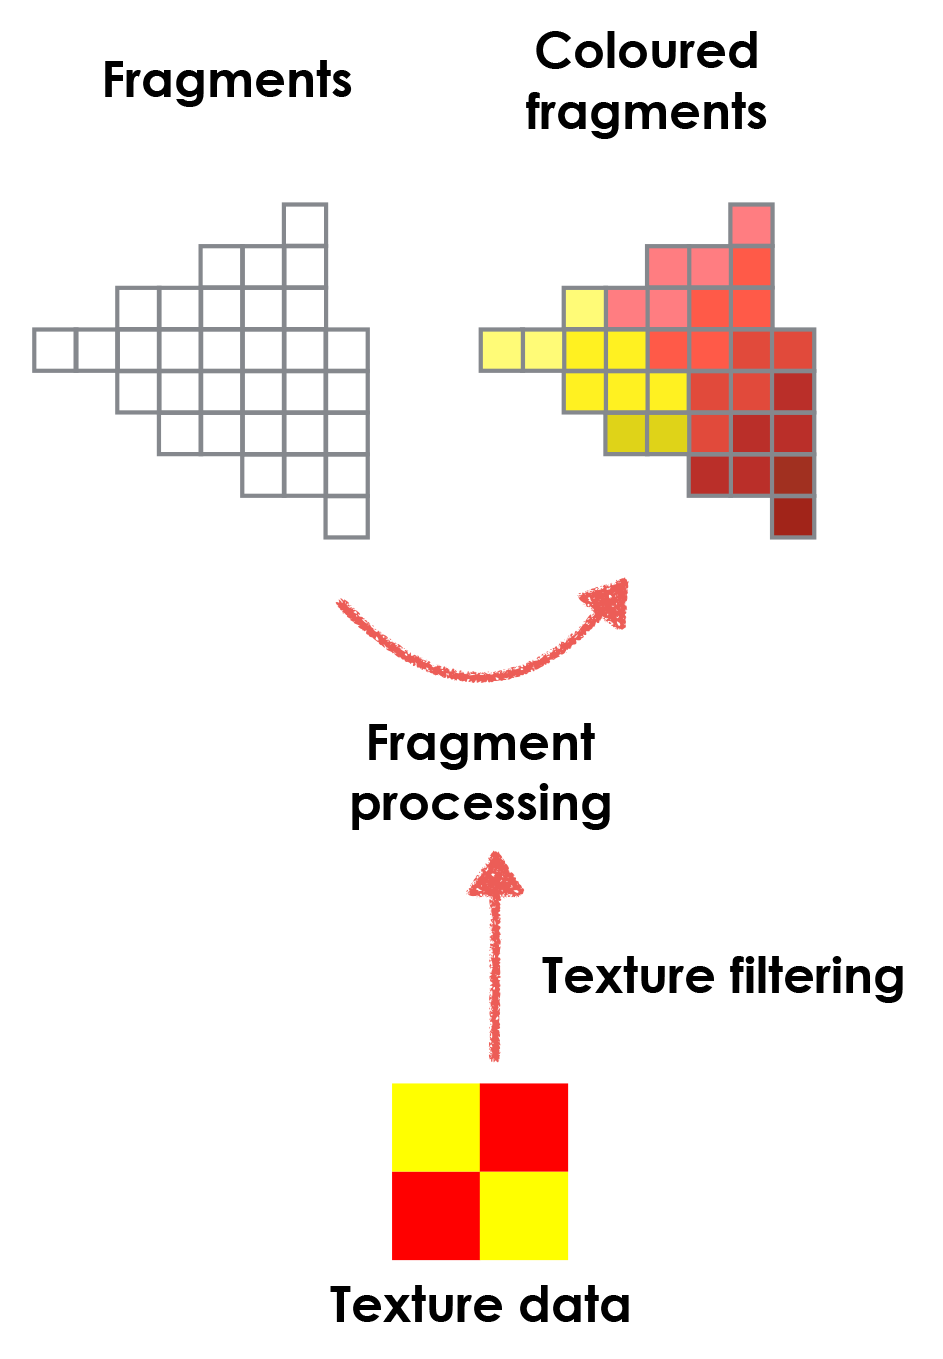
\includegraphics[width=\textwidth]{pipeline_3}
\end{column}
\begin{column}{0.65\textwidth}
\begin{itemize}
\pause\item Determine the \textbf{colour} of each fragment covered by the triangle
\pause\item \textbf{Textures} are 2D images that can be \textbf{wrapped} onto a 3D object
\pause\item Colour is calculated based on \textbf{texture}, \textbf{lighting} and other
properties of the surface being rendered (e.g.\ shininess, roughness)
\end{itemize}
\end{column}
\end{columns}
\end{frame}

\begin{frame}{Blending}
\begin{columns}
\begin{column}{0.3\textwidth}
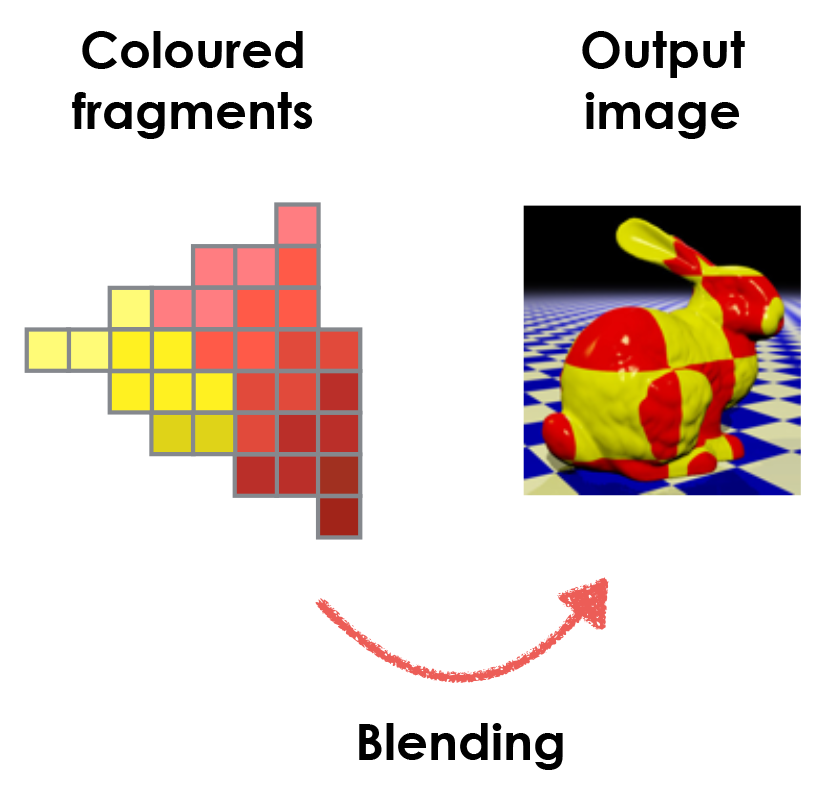
\includegraphics[width=\textwidth]{pipeline_4}
\end{column}
\begin{column}{0.65\textwidth}
\begin{itemize}
\pause\item Combine these fragments with the existing content of the image buffer
\pause\item \textbf{Depth testing}: if the new fragment is ``in front'' of the old one, replace it;
if it is ``behind'', discard it
\pause\item \textbf{Alpha blending}: combine the old and new colours for a semi-transparent appearance
\end{itemize}
\end{column}
\end{columns}
\end{frame}

\begin{frame}{Shaders}
\begin{itemize}
\item The vertex processor and fragment processor are \textbf{programmable}
\pause\item Programs for these units are called \textbf{shaders}
\pause\item \textbf{Vertex shader}: responsible for geometric transformations, deformations, and projection
\pause\item \textbf{Fragment shader}: responsible for the visual appearance of the surface
\pause\item Vertex shader and fragment shader are separate programs,
but the vertex shader can pass arbitrary values through to the fragment shader
\end{itemize}
\end{frame}
\part{Subsurface Shaders}
\frame{\partpage}


\begin{frame}{Shaders in Unity}
\end{frame}

\begin{frame}{Structure of Shaders}
\end{frame}
\part{Shading Languages}
\frame{\partpage}


\begin{frame}{High Level Shading Language (HLSL)}
\begin{itemize}
	\pause\item Used for writing \textbf{shaders} for Direct3D and Unity3D
	\pause\item C-like syntax
	\pause\item This is 
\end{itemize}
\end{frame}
\part{Subsurface Shaders}
\frame{\partpage}


\begin{frame}{Shaders in Unity}
\end{frame}

\begin{frame}{Structure of Shaders}
\end{frame}

\begin{frame}{Exercise 1 - Surface Shaders}
	\begin{itemize}
		\item Map two textures onto an object
		\item Tint the object with a colour
		\item Animate the texture coordinates for one of the textures
		\item Implement a dissolve effect
	\end{itemize}
\end{frame}

\begin{frame}{Exercise 2 - Surface Shader (Vertex Shader)}
	\begin{itemize}
		\item Add a vertex shader to the Surface Shader, ensure it carries out the standard transformation
		\item Extrude the mesh based on the Vertex Normals
		\item Animate this extrusion based
	\end{itemize}
\end{frame}

\begin{frame}{Exercise 3 - Image Effects}
\begin{itemize}
	\item Add a vignette to overlay the screen
	\item Make this vignette appear for a short time before being disabled
	\item Add a CRT TV distortion (this may require multiple Image Effects)
\end{itemize}
\end{frame}

\begin{frame}{Further Reading}
	\begin{itemize}
		\item Shaders Overview - \url{https://docs.unity3d.com/Manual/ShadersOverview.html}
		\item Gentle Introduction to Shaders - \url{http://www.alanzucconi.com/2015/06/10/a-gentle-introduction-to-shaders-in-unity3d/}
		\item HLSL Language Syntax - \url{https://msdn.microsoft.com/en-us/library/windows/desktop/bb509615(v=vs.85).aspx}
		\item HLSL Intrinsic Functions - \url{https://msdn.microsoft.com/en-us/library/windows/desktop/ff471376(v=vs.85).aspx} 
	\end{itemize}
\end{frame}
\end{document}